\documentclass[a4paper]{article}

%\renewcommand*{\sectfont}{\normalfont\bfseries}

\usepackage{fixltx2e}
\usepackage{isomath}

\usepackage[utf8]{inputenc}
\usepackage[T1]{fontenc}
\usepackage[british]{babel}

\makeatletter
\useshorthands{"}%
\defineshorthand{"-}{\nobreak-\bbl@allowhyphens}
\defineshorthand{"=}{\nobreak--\bbl@allowhyphens}
\makeatother

\usepackage{amsmath}
\usepackage{amsfonts}
\usepackage{natbib}
\usepackage{proof}
\usepackage{tikz}
\usetikzlibrary{calc}
\usepackage{url}

\usepackage{microtype}

\usepackage{hyperref}

\newcommand*{\INFER}[3][]{\ensuremath{\infer[\text{\footnotesize #1}]{\mathstrut #2}{\mathstrut #3}}}

\newcommand*{\GRAPHR}[2]{%
	\begin{tikzpicture}[xscale=0.5, yscale=0.5]
		\path[draw, white] (0, 0) rectangle (1, 1);
		\path[thick, ->] (0, 0) edge[out=90, in=90, looseness=3] (1, 0);
		\node[anchor=north] at (0, 0) {$\mathstrut #1$};
		\node[anchor=north] at (1, 0) {$\mathstrut #2$};
	\end{tikzpicture}%
}

\newcommand*{\GRAPHL}[2]{%
	\begin{tikzpicture}[xscale=0.5, yscale=0.5]
		\path[draw, white] (0, 0) rectangle (1, 1);
		\path[thick, <-] (0, 0) edge[out=90, in=90, looseness=3] (1, 0);
		\node[anchor=north] at (0, 0) {$\mathstrut #1$};
		\node[anchor=north] at (1, 0) {$\mathstrut #2$};
	\end{tikzpicture}%
}

\newcommand*{\GRAPHH}[2]{%
	\begin{tikzpicture}[xscale=0.5, yscale=0.5]
		\path[draw, white] (0, 0) rectangle (1, 1);
		\draw[thick, help lines] (0, 0) rectangle (1, 0.75);
		\node[anchor=north] at (0, 0) {$\mathstrut #1$};
		\node[anchor=north] at (1, 0) {$\mathstrut #2$};
	\end{tikzpicture}%
}

\newcommand*{\SEQR}[2]{%
	\begin{tikzpicture}[xscale=0.5, yscale=0.5]
		\path[draw, white] (0, 0) rectangle (3.5, 1);
		\path[thick, ->] (0, 0) edge[out=90, in=90, looseness=3] (1, 0);
		\path[thick, ->] (2.5, 0) edge[out=90, in=90, looseness=3] (3.5, 0);
		\node at (1.75, 0.5) {$\mathstrut\cdots$};
		\node[anchor=north] at (0, 0) {$\mathstrut #1$};
		\node[anchor=north] at (3.5, 0) {$\mathstrut #2$};
	\end{tikzpicture}%
}

\newcommand*{\SEQL}[2]{%
	\begin{tikzpicture}[xscale=0.5, yscale=0.5]
		\path[draw, white] (0, 0) rectangle (3.5, 1);
		\path[thick, <-] (0, 0) edge[out=90, in=90, looseness=3] (1, 0);
		\path[thick, <-] (2.5, 0) edge[out=90, in=90, looseness=3] (3.5, 0);
		\node at (1.75, 0.5) {$\mathstrut\cdots$};
		\node[anchor=north] at (0, 0) {$\mathstrut #1$};
		\node[anchor=north] at (3.5, 0) {$\mathstrut #2$};
	\end{tikzpicture}%
}

\newcommand*{\SEQM}[2]{%
	\begin{tikzpicture}[xscale=0.5, yscale=0.5]
		\path[draw, white] (0, 0) rectangle (3.5, 1);
		\path[thick] (0, 0) edge[out=90, in=90, looseness=3] (1, 0);
		\path[thick] (2.5, 0) edge[out=90, in=90, looseness=3] (3.5, 0);
		\node at (1.75, 0.5) {$\mathstrut\cdots$};
		\node[anchor=north] at (0, 0) {$\mathstrut #1$};
		\node[anchor=north] at (3.5, 0) {$\mathstrut #2$};
	\end{tikzpicture}%
}

\newcommand*{\SEQU}[2]{%
	\begin{tikzpicture}[xscale=0.5, yscale=0.5]
		\path[draw, white] (0, 0) rectangle (3.5, 1);
		\path[thick] (0, 0) edge[out=90, in=90, looseness=3] (1, 0);
		\path[thick] (2.5, 0) edge[out=90, in=90, looseness=3] (3.5, 0);
		\node at (1.75, 0.5) {$\mathstrut\cdots$};
		\node at (1.75, 0.5) {$//$};
		\node[anchor=north] at (0, 0) {$\mathstrut #1$};
		\node[anchor=north] at (3.5, 0) {$\mathstrut #2$};
	\end{tikzpicture}%
}

\linespread{1.1}

\newcommand*{\ALGEBRA}[1]{\mathfrak{#1}}
\newcommand*{\FUN}[1]{\text{#1}}
\newcommand*{\SET}[1]{\{#1\}}
\newcommand*{\SETC}[2]{\SET{\,#1\mid #2\,}}
\newcommand*{\TERMS}[1]{T({#1})}

\begin{document}

\title{Tabulation of Noncrossing Acyclic Digraphs}

\author{%
	Marco Kuhlmann\\
	Department of Computer and Information Science\\
	Linköping University, Sweden}

\maketitle


\section{Introduction}

\begin{figure}
	\centering\footnotesize
	\input ncdags-examples
	\caption{Some (out of 335) noncrossing acyclic digraphs of size~4.}
	\label{fig:ncdags-examples}
\end{figure}

A \emph{noncrossing graph} of size $n$ is a graph drawn on $n$ (labelled) vertices on a circle such that the edges are straight"-line segments that do not cross.
In this note I am concerned with \emph{noncrossing acyclic digraphs}.
(Examples of such structures are given in Figure~\ref{fig:ncdags-examples}.)
I present an $O(n^3)$"-time algorithm that produces an $O(n^2)$"-space representation of the set of all noncrossing acyclic digraphs of a given size~$n$.
This representation can be used as the basis for a wide range of dynamic programming algorithms on these graphs.
As an illustration, along with this note I am releasing the implementation of an algorithm for counting the number of noncrossing acyclic digraphs of a given size.\footnote{\url{https://github.com/khlmnn/ncdags}}
The corresponding integer sequence (starting with $n = 1$) is \citep{tirrell2014number}:
\begin{center}
	1, 3, 25, 335, 5521, 101551, 1998753, 41188543, 877423873, 19166868607, \dots
\end{center}
Another application of the tabulation technique is in semantic dependency parsing \citep{oepen2014broad}, where it can be used to compute the highest"-scoring dependency graph for a given sentence under an edge"-factored model.


\section{Preliminaries}

Before presenting the tabulation, I introduce some terminology and intuitions that will be useful for its understanding.

\subsection{Terminology}
\label{sec:Terminology}

In a noncrossing acyclic digraph, an edge $i \to j$ is called \emph{left"-to"-right} if $i < j$, and \emph{right"-to"-left} if $j < i$.
A graph is called \emph{edge"-covered} if there is an edge (either left"-to"-right or right"-to"-left) connecting its extremal vertices.
If a graph is not edge"-covered, we may distinguish two cases, depending on whether or not the graph is weakly connected, that is, whether there exists a path (of two or more edges) between the extremal vertices.
In the following, we use the term \emph{connected} in the sense `weakly connected but not edge"-covered'.
For connected graphs, we may additionally distinguish three cases:
\begin{enumerate}
	\item There is a directed path from the leftmost vertex to the rightmost vertex. In this case, we say that the graph is \emph{R-connected}.
	\item There is a directed path from the rightmost vertex to the leftmost vertex. In this case, we say that the graph is \emph{L-connected}.
	\item There is no directed path between the two extremal vertices. In this case, we say that the graph is \emph{N-connected}.
\end{enumerate}
Finally, even for graphs that are neither edge"-covered nor weakly connected, we may distinguish two cases, depending on whether the graph is of size~$2$ or of size greater than~$2$.
In the former case, the graph is uniquely determined; it is the graph with two nodes and no edges.
We refer to this graph as the \emph{elementary graph}, and to graphs of size greater than~$2$ as \emph{non"-elementary}.

\subsection{Algebraic Structure}

The proposed tabulation is based on a specific algebraic view on noncrossing acyclic digraphs.
Under this view, every graph is composed from the elementary graph by means of the following operations:
\begin{itemize}
	\item The first operation \emph{concatenates} two graphs, identifying the last vertex of the first graph with the first vertex of the second graph. This operation is best visualized when drawing the graphs on a straight line rather than on a circle. (With this layout, the non"-crossing condition means that the edges can be drawn in the half"-plane above the line without crossings.)
	\begin{displaymath}
		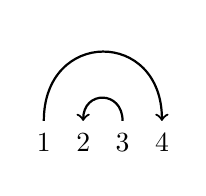
\begin{tikzpicture}[xscale=0.5, baseline=(n1.north)]
			\node (n1) at (0, 0) {$\mathstrut 1$};
			\node (n2) at (1, 0) {$\mathstrut 2$};
			\node (n3) at (2, 0) {$\mathstrut 3$};
			\node (n4) at (3, 0) {$\mathstrut 4$};
			\path[thick, ->] (n1) edge[out=90, in=90] (n4);
			\path[thick, ->] (n3) edge[out=90, in=90] (n2);
		\end{tikzpicture}
		\quad\text{concatenated with}\quad
		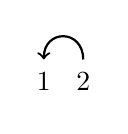
\begin{tikzpicture}[xscale=0.5, baseline=(n1.north)]
			\node (n1) at (0, 0) {$\mathstrut 1$};
			\node (n2) at (1, 0) {$\mathstrut 2$};
			\path[thick, ->] (n2) edge[out=90, in=90] (n1);
		\end{tikzpicture}
		\quad\text{yields}\quad
		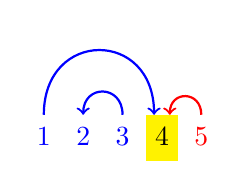
\begin{tikzpicture}[xscale=0.5, baseline=(n1.north)]
			\node[blue] (n1) at (0, 0) {$\mathstrut 1$};
			\node[blue] (n2) at (1, 0) {$\mathstrut 2$};
			\node[blue] (n3) at (2, 0) {$\mathstrut 3$};
			\node[fill=yellow] (n4) at (3, 0) {$\mathstrut 4$};
			\node[red] (n5) at (4, 0) {$\mathstrut 5$};
			\path[thick, ->, blue] (n1) edge[out=90, in=90] ($(n4.north) - (0.2, 0)$);
			\path[thick, ->, blue] (n3) edge[out=90, in=90] (n2);
			\path[thick, ->, red] (n5) edge[out=90, in=90] ($(n4.north) + (0.2, 0)$);
		\end{tikzpicture}
	\end{displaymath}
	Here the vertices and edges contributed by the first graph are drawn in blue, those contributed by the second graph are drawn in red, and the joint vertex (simultaneously the last vertex of the first graph and the first vertex of the second graph) is highlighted in yellow.
	
	\item The second and the third operation \emph{cover} a graph by adding a new edge between the first vertex and the last vertex. In the following illustration, the new edges are drawn in red:
	\begin{displaymath}
		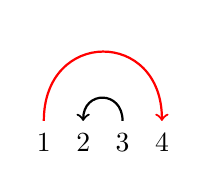
\begin{tikzpicture}[xscale=0.5]
			\node (n1) at (0, 0) {$\mathstrut 1$};
			\node (n2) at (1, 0) {$\mathstrut 2$};
			\node (n3) at (2, 0) {$\mathstrut 3$};
			\node (n4) at (3, 0) {$\mathstrut 4$};
			\path[thick, ->, red] (n1) edge[out=90, in=90] (n4);
			\path[thick, ->] (n3) edge[out=90, in=90] (n2);
		\end{tikzpicture}
		\qquad
		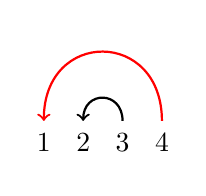
\begin{tikzpicture}[xscale=0.5]
			\node (n1) at (0, 0) {$\mathstrut 1$};
			\node (n2) at (1, 0) {$\mathstrut 2$};
			\node (n3) at (2, 0) {$\mathstrut 3$};
			\node (n4) at (3, 0) {$\mathstrut 4$};
			\path[thick, <-, red] (n1) edge[out=90, in=90] (n4);
			\path[thick, ->] (n3) edge[out=90, in=90] (n2);
		\end{tikzpicture}
	\end{displaymath}
\end{itemize}

Note that the cover operations may introduce cycles, and even multiple edges.
I shall return to this point in the next section.


\section{Inference System}

I now present the proposed tabulation for noncrossinga acyclic digraphs, specified in terms of a deduction system \citep{shieber1995principles}.
To simplify the presentation, I focus on graphs of size $n \geq 2$.

\subsection{Items}

Following the classification given in Section~\ref{sec:Terminology}, the items of the deduction system take one of seven possible forms.
\begin{itemize}
	\item \textit{Items for edge"-covered graphs.}
	\begin{displaymath}
		\GRAPHR{i}{j}
		\qquad
		\GRAPHL{i}{j}
	\end{displaymath}
	The intended meaning of these items is: `It is possible to construct an edge"-covered noncrossing acyclic digraph on the segment $[i, j]$.'
	
	\item \textit{Items for connected graphs.}
	\begin{displaymath}
		\SEQR{i}{j}
		\qquad
		\SEQL{i}{j}
		\qquad
		\SEQM{i}{j}
	\end{displaymath}
	The intended meaning of these items is: `It is possible to construct an R"-connected, L"-connected, N"-connected noncrossing acyclic digraph on the segment $[i, j]$.'
	
	\item \textit{Items for unconnected graphs.}
	\begin{displaymath}
		\SEQU{i}{j}
	\end{displaymath}
	The intended meaning of these items is: `It is possible to construct an unconnected (but not edge"-covered) noncrossing acyclic digraph on the segment $[i, j]$.'
	
	\item Finally, there are the items for the elementary graphs:
	\begin{displaymath}
		\GRAPHH{i}{j}
	\end{displaymath}
\end{itemize}

\subsection{Axioms}

The axioms of the deduction system are the items for the elementary graphs.

\subsection{Rules}

We now present the rules of our deduction system.

\paragraph{Concatenate two edge"-covered graphs}

The first four rules simulate the concatenation of two edge"-covered graphs.
The result of such a concatenation is not edge"-covered but connected:
\begin{displaymath}
	\INFER[01]{\SEQR{i}{k}}{\GRAPHR{i}{j} & \GRAPHR{j}{k}}
	\quad
	\INFER[02]{\SEQL{i}{k}}{\GRAPHL{i}{j} & \GRAPHL{j}{k}}
	\quad
	\INFER[03]{\SEQM{i}{k}}{\GRAPHR{i}{j} & \GRAPHL{j}{k}}
	\quad
	\INFER[04]{\SEQM{i}{k}}{\GRAPHL{i}{j} & \GRAPHR{j}{k}}
\end{displaymath}

\paragraph{Concatenate an edge"-covered graph and the elementary graph}

The next rules simulate the concatenation of an edge"-covered graph and the elementary graph.
The result of such a concatenation is neither edge"-covered nor connected.
There are four cases:
\begin{displaymath}
	\INFER[05]{\SEQU{i}{k}}{\GRAPHR{i}{j} & \GRAPHH{j}{k}}
	\quad
	\INFER[06]{\SEQU{i}{k}}{\GRAPHH{i}{j} & \GRAPHR{j}{k}}
	\quad
	\INFER[07]{\SEQU{i}{k}}{\GRAPHL{i}{j} & \GRAPHH{j}{k}}
	\quad
	\INFER[08]{\SEQU{i}{k}}{\GRAPHH{i}{j} & \GRAPHL{j}{k}}
\end{displaymath}

\paragraph{Concatenate a connected graph and an edge"-covered graph}

The following rules simulate the concatenation of a connected graph and an edge"-covered graph.
The result of such a concatenation is not edge"-covered but connected.
There are 6 cases; we group these cases based on the type of the first argument of the concatenation operation.

\begin{trivlist}
	\item\relax \textit{Group~1: The first argument is R"-connected}
	\begin{displaymath}
		\INFER[09]{\SEQR{i}{k}}{\SEQR{i}{j} & \GRAPHR{j}{k}}
		\qquad
		\INFER[10]{\SEQM{i}{k}}{\SEQR{i}{j} & \GRAPHL{j}{k}}
	\end{displaymath}
	
	\item\relax \textit{Group~2: The first argument is L"-connected}
	\begin{displaymath}
		\INFER[11]{\SEQM{i}{k}}{\SEQL{i}{j} & \GRAPHR{j}{k}}
		\qquad
		\INFER[12]{\SEQL{i}{k}}{\SEQL{i}{j} & \GRAPHL{j}{k}}
	\end{displaymath}
	
	\item\relax \textit{Group~3: The first argument is U"-connected}
	\begin{displaymath}
		\INFER[13]{\SEQM{i}{k}}{\SEQM{i}{j} & \GRAPHR{j}{k}}
		\qquad
		\INFER[14]{\SEQM{i}{k}}{\SEQM{i}{j} & \GRAPHL{j}{k}}
	\end{displaymath}
\end{trivlist}

\paragraph{Concatenate a connected graph and the elementary graph}

The next rules simulate the concatenation of a connected graph and the elementary graph.
The result of such a concatenation is an unconnected graph.
There are 3~cases:
\begin{displaymath}
	\INFER[15]{\SEQU{i}{k}}{\SEQR{i}{j} & \GRAPHH{j}{k}}
	\quad
	\INFER[16]{\SEQU{i}{k}}{\SEQL{i}{j} & \GRAPHH{j}{k}}
	\quad
	\INFER[17]{\SEQU{i}{k}}{\SEQM{i}{j} & \GRAPHH{j}{k}}
\end{displaymath}

\paragraph{Concatenate to an unconnected graph}

The next rules simulate the concatenation to an unconnected graph.
The result of such a concatenation is another unconnected graph.
We only need to consider concatenations where the second argument is either edge"-covered or the elementary graph:
\begin{displaymath}
	\INFER[18]{\SEQU{i}{k}}{\SEQU{i}{j} & \GRAPHR{j}{k}}
	\quad
	\INFER[19]{\SEQU{i}{k}}{\SEQU{i}{j} & \GRAPHL{j}{k}}
	\quad
	\INFER[20]{\SEQU{i}{k}}{\SEQU{i}{j} & \GRAPHH{j}{k}}
\end{displaymath}

\paragraph{Cover a graph}

The rules in the final group simulate the covering operation.
The result of such an operation is an edge"-covered graph.
There are 6~cases; we group them based on the direction of the covering edge.
\begin{trivlist}
	\item\relax \textit{Group~1: The covering edge is left"-to"-right}
	\begin{displaymath}
		\INFER[21]{\GRAPHR{i}{j}}{\SEQR{i}{j}}
		\qquad
		\INFER[22]{\GRAPHR{i}{j}}{\SEQM{i}{j}}
		\qquad
		\INFER[23]{\GRAPHR{i}{j}}{\SEQU{i}{j}}
	\end{displaymath}
	
	\item\relax \textit{Group~2: The covering edge is right"-to"-left}
	\begin{displaymath}
		\INFER[24]{\GRAPHL{i}{j}}{\SEQL{i}{j}}
		\qquad
		\INFER[25]{\GRAPHL{i}{j}}{\SEQM{i}{j}}
		\qquad
		\INFER[26]{\GRAPHL{i}{j}}{\SEQU{i}{j}}
	\end{displaymath}
\end{trivlist}

\subsection{Properties}

sound, complete, unique derivations


\section*{Acknowledgments}

The decomposition that is the basis for the tabulation presented in this note was inspired by a counting technique for noncrossing acyclic digraphs proposed by \citet{tirrell2014number}.


\bibliographystyle{plainnat}
\bibliography{mcqm}

\end{document}
